\chapter{\'{E}TAT DE L’ART} \label{intro}
%------------------------------------------
\section{Introduction}
    Dans ce chapitre nous allons présenter un état de l’art sur le Cloud Computing.
    Nous commencerons  en premier temps par introduire le concept de Cloud Computing.
    Suite à cela nous aborderons les différentes couches qui constituent le Cloud.
    Ensuite nous présenterons les différents types de déploiements du Cloud.
    Enfin nous allons terminer par définir ce qu’est une ontologie et l’avantage d’avoir recours à une ontologie du Cloud dans le mécanisme de recherche.

\section{Concepts Fondamentaux}
    \subsection{Cloud Computing}
        \subsubsection{1.2.1.1 Définition et apport}


                Le Cloud computing repose sur le partage des ressources pour atteindre la cohérence et les économies d'échelle, semblable à un utilitaire (comme le réseau d'électricité) sur un réseau .Il est à la base  d’une large infrastructure convergée et partagé de services.\\

                Cloud computing, ou également appellé "le nuage informatique", met également l'accent sur la maximisation de l'efficacité des ressources partagées. Les nuages de ressources sont généralement non seulement partagé par plusieurs utilisateurs, mais sont également réaffectées dynamiquement selon la demande. Par exemple, un centre informatique en nuage qui sert les utilisateurs européens pendant les heures d'affaires avec une application spécifique (par exemple, e-mail) peut réaffecter les mêmes ressources pour servir les utilisateurs d'Amérique du Nord avec une autre application (par exemple, un serveur Web) . Cette approche devrait permettre de maximiser l'utilisation de la puissance de calcul en réduisant ainsi les dommages environnementaux ainsi  que la dépense  d'énergie, climatisation, etc…  Avec le cloud computing, plusieurs utilisateurs peuvent accéder à un seul serveur pour récupérer et mettre à jour leurs données sans avoir à acheter des licences pour des applications différentes.\\

                Il est le résultat de l'évolution et l'adoption de technologies et des paradigmes existants. Son objectif est de permettre aux utilisateurs de tirer profit de l'ensemble de ces technologies, sans avoir besoin de connaissances approfondies dans le  sujet ou de l'expertise avec chacun d'entre eux. Le nuage a pour objectif de réduire les coûts, et aide les utilisateurs à se concentrer sur leur cœur de métier plutôt que d'être entravé par des obstacles informatiques. \\

                La principale technologie habilitante pour le cloud computing est la virtualisation. Les logiciels de virtualisation séparent un dispositif informatique physique dans un ou plusieurs dispositifs «virtuels», chacun pouvant être facilement utilisé et géré pour effectuer des tâches informatiques. La virtualisation au niveau du système d'exploitation permet la création d’un système évolutif qui optimise l’allocation des ressources inactives et ainsi améliore drastiquement la performance et l’économie d’énergie. La virtualisation offre l'agilité nécessaire pour accélérer les opérations informatiques, et réduit le coût en augmentant l'utilisation de l'infrastructure.\\
                L’Informatique autonome permet d’automatiser le processus par lequel les ressources utilisateurs sont approvisionnés. En minimisant la participation des utilisateurs, l’automatisation accélère le processus, réduit les coûts de main-d'œuvre et réduit la possibilité d'erreurs humaines.\\


                Le Cloud computing adopte des concepts de l'architecture orientée services SOA qui peuvent aider l'utilisateur à briser ces problèmes dans des services qui peuvent être intégrés pour fournir une solution. Il fournit toutes ces ressources comme des services, et fait usage des normes bien établies et des meilleures pratiques acquises dans le domaine de l'architecture SOA pour permettre un accès mondial et facile aux services du cloud computing de manière standardisée.

                Le Cloud computing exploite également des concepts de l'informatique utilitaire afin de fournir des données pour les services utilisés. Ces mesures sont à la base des modèles Cloud public pay-per-use. En outre, les services mesurés sont une partie essentielle de la boucle de rétroaction dans l'informatique autonome, permettant des services à l'échelle, à la demande pouvant être récupérés en cas de panne  automatique .\\

                C'est une sorte de grille de calcul qui  a évolué en abordant la QoS (qualité de service) et des problèmes de fiabilité. Et fournit les outils et les technologies pour construire des données / calculer  des applications parallèles intensives avec des prix beaucoup plus abordables par rapport aux techniques traditionnelles de calcul parallèle.\\

                Le Cloud computing partage des caractéristiques avec:
            \begin{itemize}
                \item[\quad $\bullet$]Modèle client-serveur :client-serveur informatique se réfère largement à toute application distribuée qui distingue entre les prestataires de services (serveurs) et les demandeurs de services (clients).
                \item[\quad $\bullet$]Grid computing : Une forme de calcul distribué et parallèle, par laquelle un« super-ordinateur et virtuel »est composé d'un groupe d'ordinateurs en réseau, faiblement couplés agissant pour réaliser de très grandes tâches.
                \item[\quad $\bullet$]Mainframe informatique : ordinateurs puissants utilisés principalement par les grandes organisations pour les applications critiques, généralement des données en vrac de traitement tels que: recensement; statistiques de l'industrie et de la consommation; la police et les services secrets de renseignement; progiciel de gestion intégré et traitement des transactions financières.
                \item[\quad $\bullet$]L'informatique utilitaire : Emballages de ressources informatiques, tels que calcul et de stockage, comme un service mesurée semblable à un service public traditionnel, comme l'électricité.
                \item[\quad $\bullet$]Peer-to-peer - Une architecture distribuée sans la nécessité d'une coordination centrale. Les participants sont à la fois les fournisseurs et les consommateurs des ressources (en contraste avec le modèle client-serveur traditionnelle).
            \end{itemize}
            Cloud computing présente les principales caractéristiques suivantes:\\
            \begin{itemize}
                \item[\quad $\bullet$]Une grande Agilité qui améliore la capacité des utilisateurs à redistribuer les ressources d'infrastructure technologique.\\
                \item[\quad $\bullet$]L'indépendance des dispositifs et des emplacements  permettent aux utilisateurs d'accéder à des systèmes utilisant un navigateur web indépendamment de leur emplacement ou de ce dispositif qu'ils utilisent (par exemple, PC, téléphone mobile). Comme l'infrastructure est hors site (généralement fournie par un tiers) et accessible via Internet, les utilisateurs peuvent se connecter à partir de n'importe où.
                \item[\quad $\bullet$]La maintenance des applications de cloud computing est plus facile, parce qu'ils ne doivent pas nécessairement être installés sur l'ordinateur de chaque utilisateur et peuvent être accessibles à partir de différents endroits.
                \item[\quad $\bullet$]Permet le partage des ressources et des coûts à travers une grande bibliothèque d'utilisateurs permettant ainsi la centralisation de l'infrastructure dans des endroits avec des coûts inférieurs (tels que l'immobilier, l'électricité, etc.)
                \item[\quad $\bullet$]Fiabilité améliorée avec l'utilisation de plusieurs sites redondants, ce qui rend la conception du cloud computing approprié pour la continuité d'activité.
                \item[\quad $\bullet$]Évolutivité et l'élasticité ("à la demande") via le provisionnement des ressources sur une base libre-service  en temps quasi-réel.
            \end{itemize}
            La sécurité peut être améliorée grâce à la centralisation des données, les ressources axées sur la sécurité accrues, etc., mais des inquiétudes persistent à propos de  perte de contrôle sur certaines données sensibles, et le manque de sécurité pour les noyaux stockées. La sécurité est souvent  meilleure que dans les autres systèmes traditionnels, en partie parce que les fournisseurs sont en mesure de consacrer des ressources à la résolution des problèmes de sécurité que de nombreux clients ne peuvent pas se permettre de les voir attaqués.  Cependant, la complexité de la sécurité est considérablement augmentée lorsque les données sont distribuées sur une zone plus large ou sur un plus grand nombre d'appareils, ainsi que dans les systèmes multi-locataires partagés par les utilisateurs indépendants. En outre, l'accès des utilisateurs à des journaux d'audit de sécurité est impossible. Les installations de cloud privé sont en partie dirigées par le désir des utilisateurs à conserver le contrôle de l'infrastructure et d'éviter de perdre le contrôle de la sécurité de l'information.
                \subsubsection{1.2.1.2 Architecture du Cloud}
            Dans ce modèle, il ya trois couches de services différents qui sont utilisés pour spécifier ce qui est provisionné, Infrastructure as a Service (IaaS), Platform as a Service (PaaS) et Software as a Service (SaaS). En outre, il ya trois autres couches qui ne sont pas fournis comme services aux usagers. \\
            \begin{figure}[H]
            \centering
            % Requires \usepackage{graphicx}
            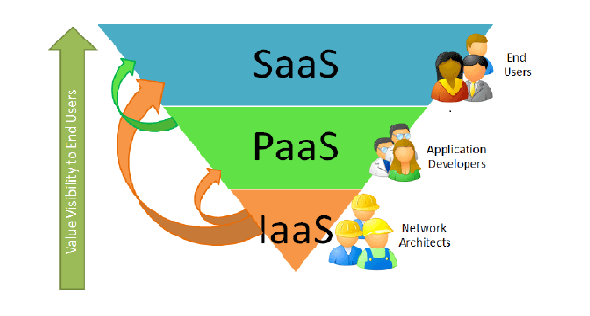
\includegraphics[width=12cm]{trois_couche_cloud}\\
             \caption{les trois couche du Cloud}\label{trois_couche_cloud}
            \end{figure}
        \begin{itemize}
            \item[\quad $\bullet$] Infrastructure as a Service (IaaS):Dans le modèle Cloud de service le plus élémentaire et selon l'IETF (Internet Engineering Task Force), les fournisseurs de IaaS offrent des ordinateurs et d'autres ressources virtuelles aux clients. Une large panoplie  d’hyperviseurs dans le système de soutien Cloud peut supporter un grand nombre de machines virtuelles et la capacité à l'échelle des services de haut en bas selon les différentes exigences des clients.) Les nuages IaaS offrent souvent des ressources supplémentaires comme une bibliothèque de machines virtuelles image disque, le stockage de bloc brut, et le fichier ou un objet de stockage, les pare-feu, les équilibreurs de charge, les adresses IP , les réseaux locaux virtuels (VLAN), des faisceaux de logiciels. Les fournisseurs IaaS-cloud fournissent ces ressources à la demande depuis leurs grandes piscines installées dans les centres de données. Pour la connectivité large zone, les clients peuvent utiliser l'Internet ou les nuages porteurs (réseaux privés virtuels dédiés).

                Pour déployer leurs applications, les utilisateurs de Cloud peuvent installer les systèmes d'exploitation de leur choix et leurs logiciels d'application sur l'infrastructure Cloud. Dans ce modèle, les correctifs et les utilisateurs de Cloud maintiennent les systèmes d'exploitation et le logiciel d'application. Les fournisseurs de Cloud facturent généralement des services IaaS sur une base informatique utilitaire: le coût reflète la quantité des ressources allouées et consommés.



                \item[\quad $\bullet$] Platform as a Service (PaaS):
                Dans les modèles PaaS, les fournisseurs de Cloud offrent une plate-forme informatique, comprenant typiquement un système d'exploitation, l'environnement d'exécution du langage de programmation, base de données, et le serveur web. Les développeurs d'applications peuvent développer et gérer leurs solutions de logiciels sur une plate-forme de Cloud sans le coût et la complexité de l'achat et la gestion des couches matérielles et logicielles sous-jacentes. Le PaaS offre des plateformes comme Microsoft Azure et Google App Engine, les ressources informatiques et de stockage sous-jacents varient automatiquement pour correspondre à la demande d'application de sorte que l'utilisateur du nuage n'a pas à allouer des ressources manuellement. Ce dernier a également été proposé par une architecture visant à faciliter en temps réel dans les environnements de cloud computing. Bien d’autres types d'applications encore plus précis peuvent être fournis par l'intermédiaire de PaaS.
.
                \item[\quad $\bullet$] Software as a Service (SaaS):
                Dans le modèle d'affaires en utilisant un logiciel comme un service (SaaS), les utilisateurs bénéficient d'un accès aux logiciels d'application et des bases de données. Les fournisseurs de Cloud gérent l'infrastructure et les plates-formes qui exécutent les applications. SaaS est parfois appelé «logiciel à la demande" et est généralement un prix sur une base pay-per-utilisation ou à l'aide d'un abonnement.\\

                Dans le modèle SaaS, les fournisseurs de Cloud installent et utilisent le logiciel d'application dans le nuage et les utilisateurs de Cloud peuvent accéder au logiciel du Cloud clients. Le Nuage d’utilisateurs ne configure  pas l'infrastructure Cloud et de plate-forme où l'application fonctionne. Ceci élimine le besoin d'installer et d'exécuter l'application sur des ordinateurs de l'utilisateur de nuages, ce qui simplifie la maintenance et de soutien. Les applications Cloud sont différentes des autres applications qui peuvent être atteints par clonage de tâches sur plusieurs machines virtuelles au moment de l'exécution pour répondre à la demande changeante de travail et leur évolutivité.. Ce processus est transparent pour l'utilisateur de nuage, qui ne voit qu’un point d'accès unique. Pour accueillir un grand nombre d'utilisateurs de Cloud computing, les applications Cloud peuvent être mutualisées, c’est à dire que toute machine sert plus d'une organisation de l'utilisateur de nuage.\\

                Le modèle de tarification pour les applications SaaS est généralement un abonnement mensuel ou annuel forfaitaire par utilisateur,  donc le prix est extensible et ajustable si les utilisateurs sont ajoutés ou supprimés à tout moment.\\

                Ses partisans affirment que le  SaaS permet à une entreprise la possibilité de réduire les coûts d'exploitation IT par l'externalisation de la maintenance matérielle et logicielle et le soutien au fournisseur de cloud. Cela permet à l'entreprise de réaffecter les opérations informatiques qui coûte plus de dépenses de matériel / logiciel et les charges de personnel, en vue d'atteindre d'autres objectifs. En outre, avec des applications hébergées au centre, des mises à jour peuvent être effectuées sans la nécessité pour les utilisateurs d'installer un nouveau logiciel. Un inconvénient de SaaS est que les données des utilisateurs sont stockées sur le serveur du fournisseur de Cloud. En conséquence, il pourrait y avoir un accès non autorisé aux données. Pour cette raison, les utilisateurs sont de plus en plus pour l'adoption de systèmes intelligents de gestion de clés tiers pour aider à sécuriser leurs données.\\
            \end{itemize}
        \subsubsection{1.2.1.3Types de Déploiment}
            on distingue trois type de déploiment de cloud selon l'emplacement des ressources physiques qui fournissent les services:
                \begin{itemize}
                    \item[\quad $\bullet$]Le Cloud privé:\\
                    Le cloud privé est un type de cloud computing qui offre des avantages similaires à cloud public, y compris l'évolutivité et en libre-service, mais à travers une architecture propriétaire. Contrairement à des clouds publics, qui fournissent des services à de multiples organisations, un cloud privé est dédié à une seule organisation.
                    \item[\quad $\bullet$]Le cloud public:\\
                    Un cloud public est fondée sur le modèle de cloud computing standard, dans lequel un prestataire de services fait des ressources, telles que les applications et le stockage, à la disposition du grand public sur Internet. Services de cloud publics peuvent être libres ou offerts sur un modèle pay-per-utilisation.
                    \item[\quad $\bullet$]Le Cloud hybride:\\
                    Cloud hybride est un environnement de cloud computing qui utilise un mélange de sur site, cloud privé et des services de cloud public à l'orchestration entre les deux plates-formes. En permettant à des charges de travail de se déplacer entre les nuages privés et publics comme les besoins informatiques et les coûts changent, cloud hybride donne aux entreprises une plus grande flexibilité et plus d'options de déploiement de données.

                \end{itemize}
                    \begin{figure}[H]
                    \centering
                    % Requires \usepackage{graphicx}
                    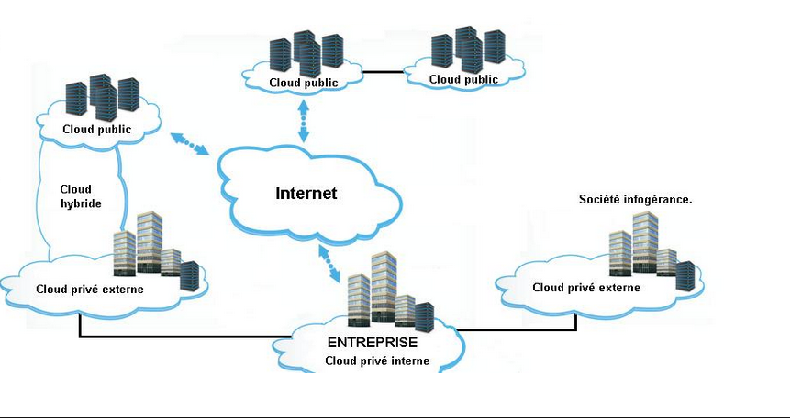
\includegraphics[width=12cm]{cloud_prive_public_hybride}\\
                    \caption{les trois couche du Cloud}\label{cloud_prive_public_hybride}
                \end{figure}
            \subsection{Ontologies}
                \subsubsection{1.2.2.1 Définition}
                     Une ontologie est une spécification explicite d’une conceptualisation d’un domaine[Gruber 1993]\\
                Elle peut fournir un vocabulaire contrôlé de concepts, chacun avec une sémantique qui est explicitement définie et compréhensible par la machine. Elle fournit également une compréhension commune d'un domaine d'intérêt pour soutenir la communication entre les ordinateurs et les humains en définissant des théories de domaine partagées. Dans le domaine de la récupération de l'information, l'ontologie qui se compose d'un ensemble de concepts et de relations entre concepts est utilisé pour traiter les requêtes des utilisateurs.\\
                Avec une ontologie Cloud, nous pouvons développer un système intelligent courtier d'adaptation qui fonctionne sur la base de la compréhension des ressources autres que les noms littéraux. Le système correspondant utilisera les connaissances à partir d'une ontologie pour raisonner sur la mesure de similarité entre les concepts autres que des termes. Dans ce contexte, le principal problème est de construire une ontologie significative dont le raisonnement est approprié pour la découverte des services Cloud. L'architecture et la mise en œuvre de notre système de découverte consiste d'agents utilisateurs, les agents de fournisseurs, et agents de correspondance .Notre approche utilise les avantages du système à base d'agents et le mécanisme d'appariement sémantique en utilisant un nuage ontologie.\\

                \subsubsection{1.2.2.2 Environnements de développement d’ontologie}
                    On trouve plusieurs éditeurs supportant tout le processus de développement des ontologies. Parmis lesquels on cite:\\
                    \begin{itemize}

                        \item[\quad $\bullet$]The Neon Toolkit : c'est un logiciel open source multiplateforme pour le développement d'ontologie. Il est basé sur la plateforme populaire Eclipse et fournit un très grand ensemble de plugins qui couvrent une varieté d'activité. \\
                        \item[\quad $\bullet$]Vitro : c'est un éditeur à usage général d'ontologie du web qui permet de créer et charger des ontologies en format OWL
                        \item[\quad $\bullet$]Protégé sous plusieurs versions qui a été développé dans Standford University\\
                    \end{itemize}
                \subsubsection{1.2.2.3 Langages de développement d’ontologies}
                Il existe plusieurs types de langage de description d'ontologies notamment:
                    \begin{itemize}
                         \item[\quad $\bullet$]Logiques de description:\\
                          langages de représentation de connaissances dont le formalisme s’appuie sur les notions de concepts, de rôles et d’instances

                         \item[\quad $\bullet$]OWL : Ontology Web Language:\\
                          Il est adopté par la recommendation W3C et utilisé comme le principal langage de représentation de connaissances basé sur XML et les logiques de description

                         \item[\quad $\bullet$]RDF: Ressource Description Framework\\
                          Il est basé sur XML et permet de représenter les connaissances sous la forme des triplets, Sujet, Prédicats, Objet

                         \end{itemize}
                \subsubsection{1.2.2.4 OWL}
                    Le langage d'ontologie Web OWL est un langage de balisage sémantique pour l'édition et le partage des ontologies sur le Web. OWL est développé comme une extension de vocabulaire de RDF (Resource Description Framework)
                    \begin{itemize}
                    \item[\quad $\bullet$]Individus : Objets particuliers du domaine
                    \item[\quad $\bullet$]Classe: un groupe d'individus partageant les mêmes caractéristiques. Les classes définies par l'utilisateur sont d'ailleurs toutes des enfants de la  super-classe OWL:Thing.
                    \item[\quad $\bullet$]Propriété : permet de définir des faits ou des relations entre ces classes. OWL fait une distinction entre :
                        \begin{itemize}
                        \item[\quad $\cdot$]Propriétés d'objet: définit une propriété entre deux individus d'une classe ou de plusieurs classes, . Exemple : hasBrother .
                        \item[\quad $\cdot$]Propriétés de données: définit une relation entre une valeur ou donnée et un individu d'une classe. Exemple : hasName.
                        \end{itemize}

                    \end{itemize}
                \section{Recherche basée sur l'ontologie et travaux existants }
                    Les mécanismes de découverte de service Cloud basée sur l'ontologie est devenu un sujet intéressant. De nombreux algorithmes, systèmes et approches ont été proposés pour assurer cette découverte. Nous allons essayer de citer les travaux les plus récents dans cette section.
                    Miranda Zhang et al. [1] ont proposé une ontologie, nommé Cocoon spécifique pour première la couche première, IaaS. Ils ont également proposé un système, CloudRecommender ayant comme objectif principal la découverte de différentes ressources offerts par cette couche. La découverte dans ce travail est limitée à la couche IaaS.
                    Nous citons également le travail de Francesco Moscato et al. [2] qui propose une API pour assurer l'interopérabilité des services multiples offerts par différents Clouds. Cela va assurer une découverte, basée sur l'ontologie, plus précise et plus intelligent.
                    Ces travaux se sont limités à la simple découverte des services Cloud. Cependant, les travaux de Sim et al. [3, 4] et Bhama et al.[5] ont utilisé la similarité dans la recherche des services Cloud. En effet, le travail de Bhama et al.[5] ont visé la nécessité de l’utilisation du raisonnement de similarité dans  la découverte des services Cloud. En effet, ils ont proposé quelques formules nécessaires à utiliser lors du recherche de service Cloud basée sur l’ontologie.
                    Sim et al. [3, 4] ont proposé Cloudle, un moteur  de recherche de service de cloud basé sur l'ontologie. Pour y faire,  Cloudle, cherche les services appropriés dans l’ontologie en utilisant la similarité et les classe selon leurs utilités, leurs prix et leurs disponibilités.
                    C’est  dans ce sens que s’oriente ce PFA. En effet, nous proposons un moteur de recherche de service Cloud basée sur l’ontologie. Plus précisément, et pour offrir à l’utilisateur final le service le plus approprié  à sa demande, nous nous basons sur la similarité des services Cloud qui est classées en trois types principaux à savoir :similarité de concepts, similarité de propriété d’objet et similarité de propriété de données. L’approche est détaillée dans le chapitre suivant.


                \section{Conclusion}

                Ce chapitre a eu pour objectif d’introduire le cadre de l’élaboration de notre projet.
                Nous avons donc présenté le Cloud Computing avec les différentes couches qui le composent et les différents type de Cloud existants et nous avons aussi introduit la notion d’ontologie et expliqué les avantages qui nous ont incités  à choisir de travailler sur l’ontologie du Cloud.
























